%第2章:準備
本章では本文中に使用する用語を述べる。

\section{諸定義}

\subsection*{V字モデル}
V字モデルとはシステム開発を要求分析、基本設計、詳細設計、実装に分けて時間軸順に検証、テストを行う開発プロセスである。細かく要素ごとにテストをしていくことで開発の途中で大幅な変更や問題が起きにくくなる利点がある。

\begin{figure}[htbp]
\centering
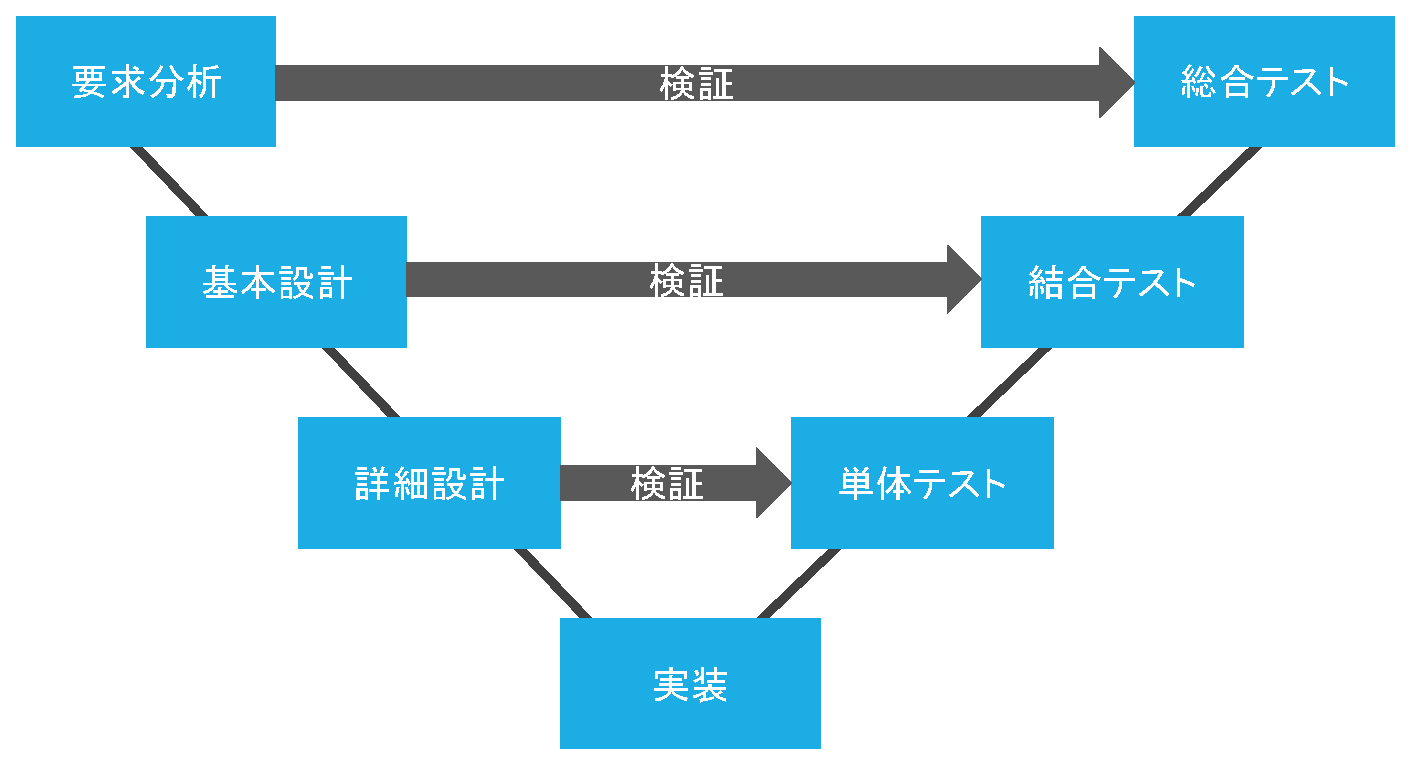
\includegraphics[width=10cm]{./pic/vjimodel.eps}
\caption{V字モデル}
\label{v_model}
\end{figure}

\subsection*{UML(Unifiled Modeling Language)}
UMLとは各開発工程で利用すべき図面を標準化した言語である。UMLの利点は、単純で分かりやすい点と、実用的な表現方法を持つ点である。UMLの構成要素としてユースケース図、クラス図、シーケンス図がある\cite{uml}。

\subsection*{ユースケース図}
システムがどのように機能すべきかという振る舞いとその外部環境を表す。


\subsection*{シーケンス図}
シーケンス図は、オブジェクト間のメッセージのやり取りを時系列順に沿って並べて表現したものである。四角の項目はオブジェクトと呼ぶ。矢印はメッセージと呼ばれ、意味はオブジェクト間のデータの伝達と動作が行われる。ユースケース図を基にしてシーケンス図やクラス図を制作を行う。

\subsection*{クラス図}
クラス図はモデルの静的な構造を示す図である。クラスが持つ動作や、属性を記述する。より具体的な実装部分に近い記述を行う。

\subsection*{Yolo(Real-Time Object Detection)}
Yoloはリアルタイムでのオブジェクト識別が可能ネットワークである。Webカメラを利用したリアルタイム検出も可能である。ほかのネットワークとの違いは、検出と識別を同時に行っているため高速性を保てる点である。今回は、画像からバーコードの位置を特定するために使用した\cite{yolo}。


\subsection*{pyzbar}
pyzbarとはバーコード画像を解析し、数字を識別するライブラリである\cite{pyzbar}。